\subsection{Model View Controller(MVC)}
In the web service component of the project we use the ASP.net MVC framework. 
This framework is using the MVC architectural pattern for structuring the code.
This pattern will be described shortly in the following, based on the overview article on the Microsoft website \citet{aspmvc}.

MVC or Model View Controller is an architectural pattern that is used to separate responsibility of an application into three parts, the model, the view, and the controller.
The pattern can be seen as an architecture diagram on \cref{mvcdiagram}

\begin{figure}[h]
\center
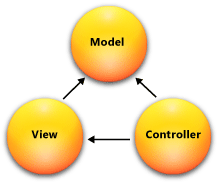
\includegraphics[width=0.4\textwidth]{graphics/mvc}
\label{mvcdiagram}
\caption{The MVC design pattern. From \cite{aspmvc}}
\end{figure}

\begin{itemize}
\item[Model] The model contains the model of the application domain and takes care of fetching data a making them available through the model.
\item[Views] Views display the model to the user.
\item[Controller] The controllers handle the interaction with users. Based on userinput the controllers work on the model and select what view needs to be used for displaying the data.
\end{itemize}